\section{Quantum Circuit and the Use of Qiskit}
%\tcbset{highlightstyle/.style={colback=yellow!10!white, colframe=orange!80!black, boxrule=0.5pt, arc=2pt, auto outer arc}}

\subsection{The quantum circuit}
\label{sec:QuantumCircuit}
\subsubsection{The Pauli Matrices}

\begin{table}[h!]
\centering
\caption{Collection of Pauli Matrices}
\label{tab:gates}
\begin{tabular}{lcr}
\toprule
Name & Symbol & Matrix Form \\
\midrule
Pauli-X & $X$ & $\begin{bmatrix}
    0&1\\1&0
\end{bmatrix}$ \\
\midrule 
Pauli-Y & $Y$ & $\begin{bmatrix}
    0&-i\\i&0
\end{bmatrix}$ \\
\midrule 
Pauli-Z & $Z$ & $\begin{bmatrix}
    1&0\\0&-1
\end{bmatrix}$ \\
\midrule 
Identity Matrix & $I$ & $\begin{bmatrix}
    1&0\\0&1
\end{bmatrix}$\\
\bottomrule
\end{tabular}
\end{table}

\subsubsection{The CNOT gate}

CNOT (Controlled-NOT) gate is the used onto two qubits: one is for controlling, the other is the target bit. Its functionality is:
\begin{itemize}
    \item \textbf{When the control bit is $\ket{1}$}, flip the target value.
    \item \textbf{When the control is $\ket{0}$}, the target is not changed.
\end{itemize}
Its matrix form is:
\begin{equation}
    CNOT=\begin{bmatrix}
    1&0&0&0\\
    0&1&0&0\\
    0&0&0&1\\
    0&0&1&0
    \end{bmatrix},
\end{equation}
corresponding to the 4D space of two qubits. Together with the Hadamard gate, CNOT can give rise to the entanglement state, known as the \textbf{Bell state}.

Howeve, in practice, if the topological structure of a quantum computer is taken into account, the realization of the CNOT from the control qubit to the target may not be straightforward. For example, as mentioned in \cite{Abhijith2018QuantumBeginner}, if qubit a is not connected to qubit c directly, say qubit b is the bridge qubit connect both of them, like the figure beow:
\begin{figure}[ht]
\centering
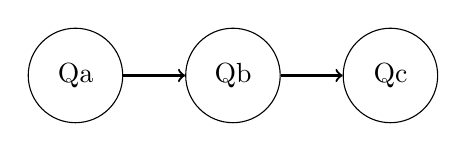
\begin{tikzpicture}[node distance=2cm, every node/.style={circle, draw, minimum size=1.2cm}]
  \node (Qa) {Qa};
  \node[right of=Qa] (Qb) {Qb};
  \node[right of=Qb] (Qc) {Qc};

  \draw[->, thick] (Qa) -- (Qb);
  \draw[->, thick] (Qb) -- (Qc);

\end{tikzpicture}
\caption{Connectivity of Three Qubits}
\label{fig:linearConnectivity}
\end{figure}
In this scenario, $\text{CNOT}_{a\rightarrow c}$ cannot be realized directly, it must be realized via qubit b:
\begin{equation}
    \text{CNOT}_{a\rightarrow c}=\text{CNOT}_{b\rightarrow c}\text{CNOT}_{a\rightarrow b}\text{CNOT}_{b\rightarrow c}\text{CNOT}_{a\rightarrow b}.
    \label{decomCNOT}
\end{equation}
As we can see, the decompostion of $\text{CNOT}_{a\rightarrow c}$ is necessary, since we want to change the target qubit c without changing the state of ancilla qubit, which is qubit b here. Actually we can let $\ket{abc}=\ket{110}$ as the initial value of those three qubits, and if we want to obtain $\ket{111}$ via $\text{CNOT}_{a\rightarrow c}$, then the decomposition in Eq.~\ref{decomCNOT} is the only way.

\subsubsection{The CZ gate}
Its matrix form is
\begin{equation}
    CZ=\begin{bmatrix}
        1&0&0&0\\
        0&1&0&0\\
        0&0&1&0\\
        0&0&0&-1
    \end{bmatrix},
\end{equation}
and its functionality is:
\begin{itemize}
    \item when the control qubit is $\ket{1}$, $Z$ gate is exerted to the target qubit, which means the phase is flipped.
    \item When the control qubit is $\ket{0}$, the target qubit does not change.
\end{itemize}

Both CZ and CNOT can cause entanglement, and both of them can convert to each other via Hadamard gate:
\begin{equation}
    CNOT_{c,t}=(I\otimes H)\cdot CZ_{c,t}\cdot(I\otimes H),
\end{equation}
which means we can obtain CNOT gate via CZ gate and Hadamard gate.


\subsection{The Qiskit}
\begin{itemize}
    \item In Qiskit, the \tcbox[inlinebox]{TwoLocal} or \tcbox[inlinebox]{EfficientSU2} are used to construct parameterized ansatz. 
    \item In Qiskit, all the simulation can be done via \tcbox[inlinebox]{AerSimulator} to realize testing and optimization.
\end{itemize}

\subsubsection{Collection of Qiskit Code}
\begin{lstlisting}[language=Python, caption=Circuit Measurement, frame=single, label={lst:CircuitMeasure}]
from qiskit.opflow import PauliSumOp
from qiskit import QuantumCircuit, Aer, execute

# 假设你要测 H = 0.7 * ZI + 0.6 * IZ - 0.9 * ZZ
H = PauliSumOp.from_list([('ZI', 0.7), ('IZ', 0.6), ('ZZ', -0.9)])

# ansatz 电路
qc = QuantumCircuit(2)
qc.ry(0.5, 0)
qc.cx(0, 1)

# 添加测量操作（可用 Estimator 接口更高效）
\end{lstlisting}

\begin{lstlisting}[language=Python, caption=Generating Hamilton, frame=single, label={lst:HamiltonGeneration}]
from qiskit_nature.second_q.drivers import PySCFDriver
from qiskit_nature.second_q.mappers import JordanWignerMapper
from qiskit_nature.second_q.problems import ElectronicStructureProblem

# 构建分子对象
driver = PySCFDriver(atom='H .0 .0 .0; H .0 .0 .74', basis='sto3g')
problem = ElectronicStructureProblem(driver)

# 得到费米子哈密顿量
second_q_op = problem.second_q_ops()['ElectronicEnergy']

# 使用 JW 映射
mapper = JordanWignerMapper()
qubit_op = mapper.map(second_q_op)

print(qubit_op)

\end{lstlisting}

\begin{figure}[ht]
\centering
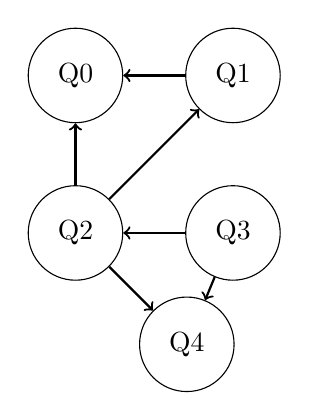
\begin{tikzpicture}[node distance=2cm, every node/.style={circle, draw, minimum size=1.2cm}]
  \node (Q0) {Q0};
  \node[right of=Q0] (Q1) {Q1};
  \node[below of=Q0] (Q2) {Q2};
  \node[below of=Q1] (Q3) {Q3};
  \node[below right of=Q2] (Q4) {Q4};

  \draw[->, thick] (Q1) -- (Q0);
  \draw[->, thick] (Q2) -- (Q0);
  \draw[->, thick] (Q2) -- (Q1);
  \draw[->, thick] (Q3) -- (Q2);
  \draw[->, thick] (Q3) -- (Q4);
  \draw[->, thick] (Q2) -- (Q4);
\end{tikzpicture}
\caption{Connectivity Graph of ibmqx4 Qubits}
\label{fig:connectivity}
\end{figure}